\chapter{Output}\label{cha:output}

Information related to the measurements (e.g. date and time, viewing angles, geolocation data,~\ldots) can be selected in the \textbf{Display} and the \textbf{Output pages} of \textbf{Projects properties}. The selected instrument or file format determines the list of fields available in this page. For example, information on cloud fraction and cloud top pressure is available only for satellite instruments. A non-exhaustive list of fields available for ground-based and satellite measurements is given in figure \ref{fig:output_fields}.

The measurement type is available for CCD EEV and MFC BIRA-IASB MAXDOAS formats.  The convention is :

\begin{itemize} \itemsep -6pt
\item 1 for off axis
\item 3 for zenith sky
\item 4 for dark currents
\item 8 for offsets
\end{itemize}

\begin{figure}
\centering
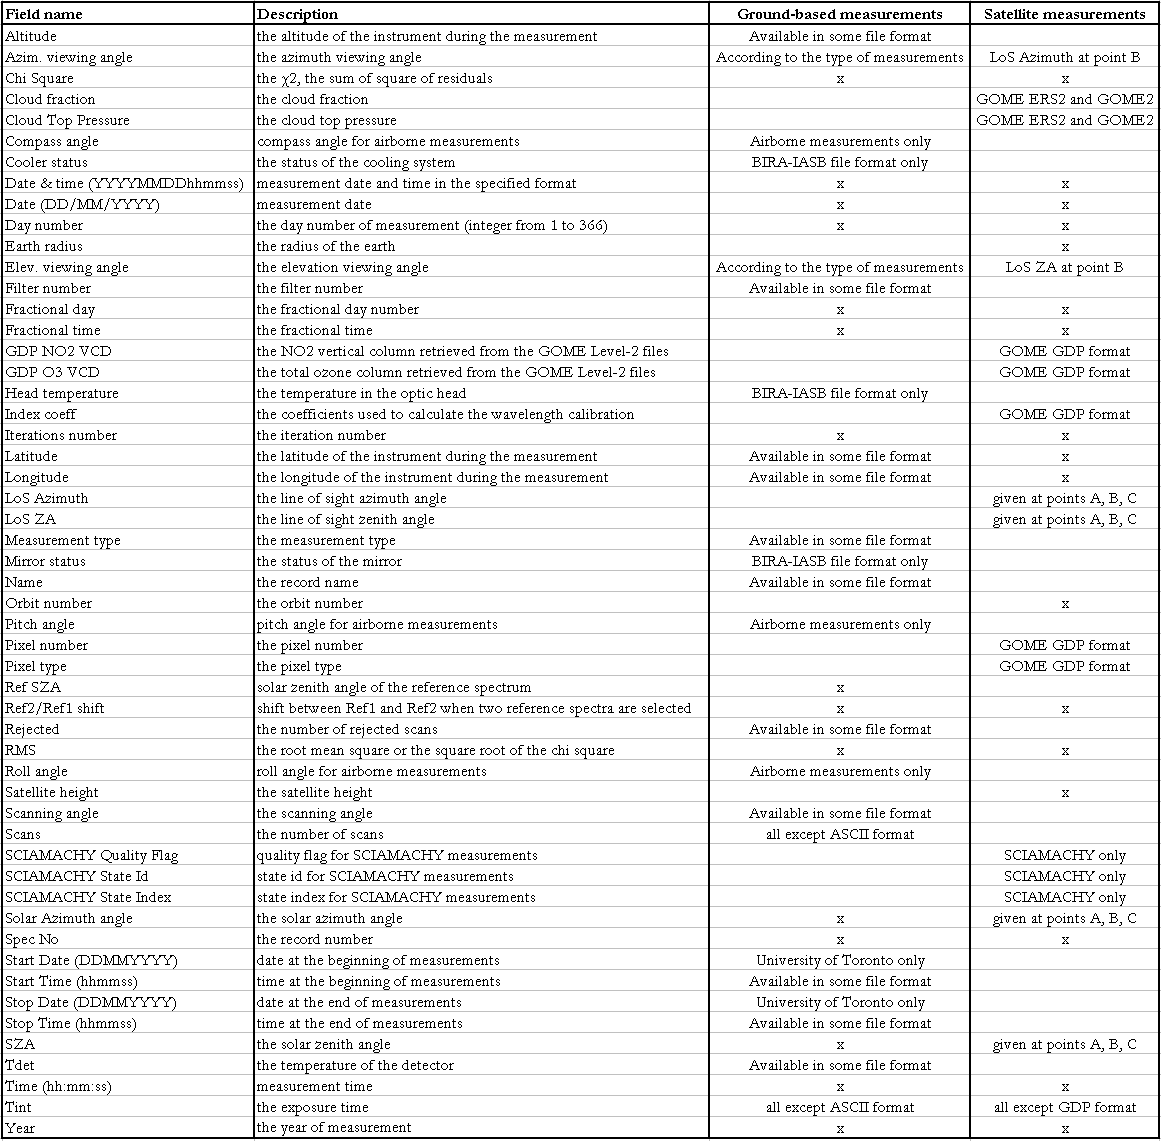
\includegraphics[width=\textwidth]{img/Output_Field.png}
\caption{A list of some of the output fields available in QDOAS.}\label{fig:output_fields}
\end{figure}

\begin{figure}
\centering
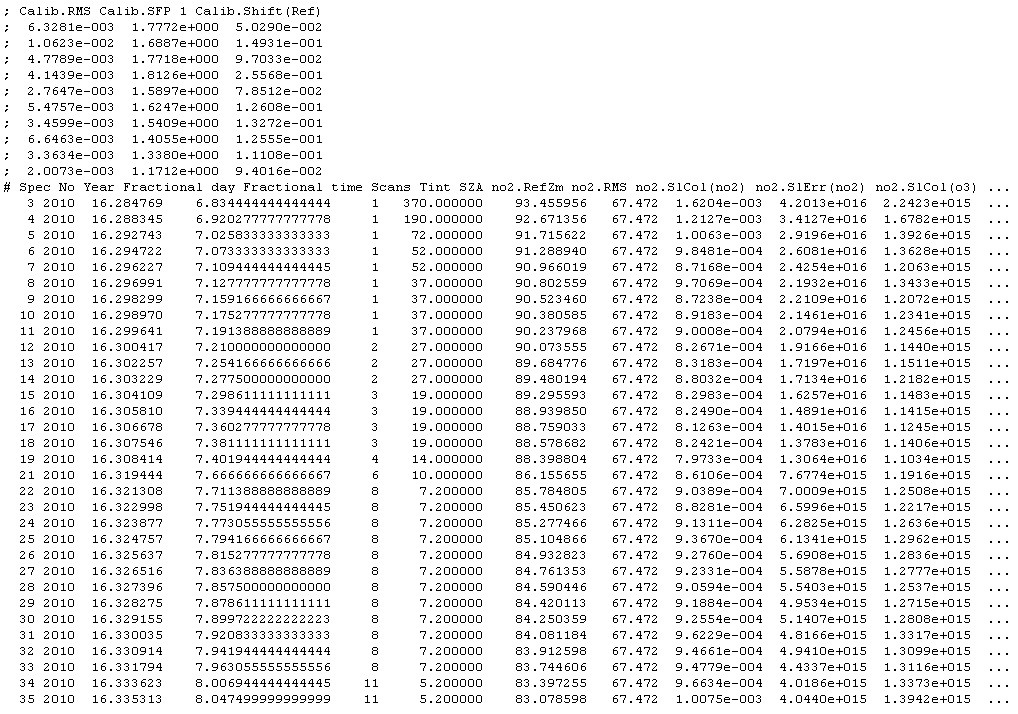
\includegraphics[width=\textwidth]{img/Output_Sample3.png}
\caption{Example of ASCII output generated by QDOAS.}\label{fig:ascii_output}
\end{figure}

In ASCII output files, columns are separated using tab characters and it is normal that they are not aligned with the column titles when the file is loaded in a simple text editor.  Figure \ref{fig:ascii_output} provides an example.  For this application, the \textbf{calibration button} is checked and results of the calibration procedure precede the analysis results. The \gls{rms}, the shift between the reference spectrum and the solar spectrum and the calculated value of the \gls{fwhm} of the fitted line shape (Gaussian in this application) for each of the sub-windows of the wavelength calibration interval are saved (see the \textbf{Calibration page} of \textbf{Projects properties} for further details).

The output in figure \ref{fig:ascii_output} contains the following fields:

\begin{enumerate} \itemsep -6pt
\item The record number (Spec No)
\item The year of measurements
\item The fractional calendar day
\item The fractional time
\item The number of scans
\item The exposure time (Tint)
\item The solar zenith angle (SZA)
\item The shift calculated between the spectrum and the reference in the no2 analysis window (no2.RefZm)
\item The \gls{rms} of the fit in the ? ``no2" analysis window (no2.RMS)
\item The slant column of \NO2 calculated in the  "no2" analysis window (no2.SlCol(no2))
\item The error on the slant column of NO2  (no2.SlErr(no2))
\item The slant column of \ozone calculated in the  ``no2" analysis window  (no2.SlCol(O3))
\item ...
\end{enumerate}

\begin{tabular}[h]{l p{3cm}}
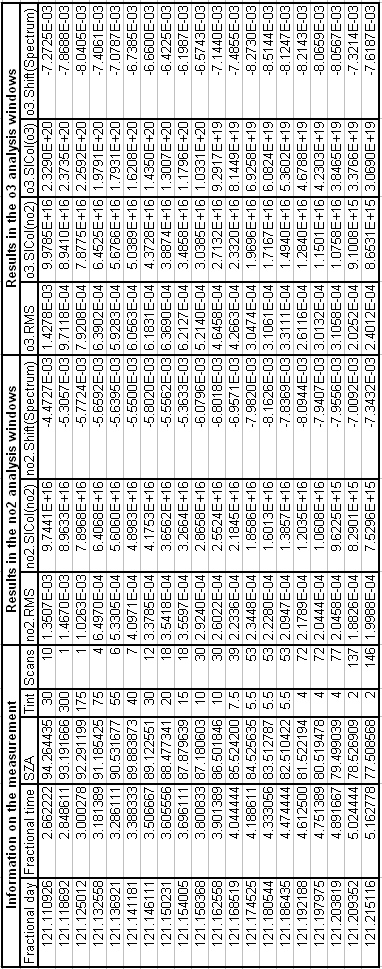
\includegraphics[height=24cm]{img/Output_Sample1.png} &
    \rotatebox{90}{\parbox{24cm}{\textbf{Example of output generated by QDOAS and loaded using Excel.} \\ In this example, only the fractional date and time, the solar zenith angle (SZA), the exposure time (Tint) and the number of scans have been selected in the \textbf{Output page} of \textbf{Projects properties}.  The application contains two analysis windows (no2 and o3).  In this example, the NO2 column has been retrieved from both no2 and o3 windows. The column title starts with the name of the analysis window.  Slant columns are indicated by \textbf{SlCol}; errors on slant columns by \textbf{SlErr} (not present in this example).}}
\end{tabular}

\begin{tabular}[h]{l p{3cm}}
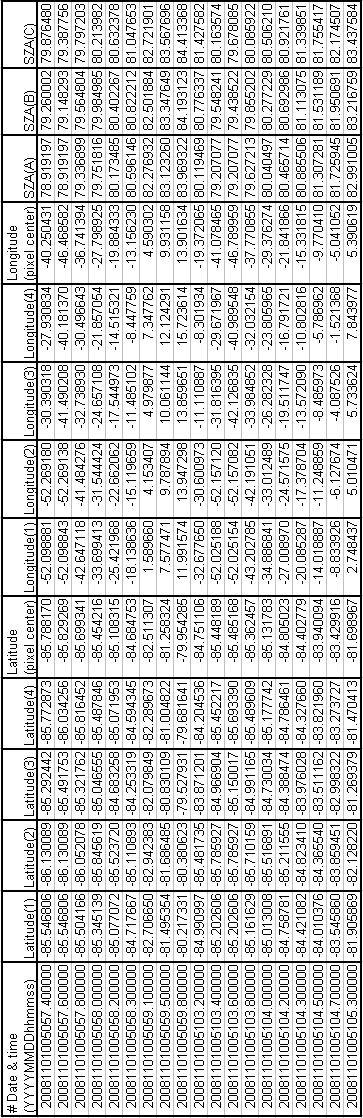
\includegraphics[height=24cm]{img/Output_Sample2.png} &
    \rotatebox{90}{\parbox{24cm}{\textbf{Example of output file generated by QDOAS and loaded using Excel.} \\ This example has been generated from a satellite application (GOME-2).  Results of the fit are not shown here.  For satellite measurements, the accuracy of the measurement time is important.  The format YYYYMMDDhhmmss (year, month, day, hour, minute, second accolated; milliseconds in the fractional part) is usually preferred to the fractional date and time.  Geolocation coordinates are given at the four corners and at the centre of the pixel. Angles such as the solar zenith angles are given at the beginning, the middle and the end of the measurement.}}
\end{tabular}


%%% Local Variables:
%%% mode: latex
%%% TeX-master: "QDOAS_manual"
%%% TeX-PDF-mode: t
%%% End:
